% !Mode:: "TeX:UTF-8"
\documentclass{beamer}

\mode<presentation>
{
\usetheme{Warsaw}

\setbeamercovered{transparent}
}

\usepackage[UTF8]{ctex} % 支持中文

% 分页Slide不编号
\setbeamertemplate{frametitle continuation}{}

% 插入多列
\usepackage{multicol}

% 插入链接
\usepackage{hyperref}
\hypersetup{urlcolor=blue}

% 插入图片
\usepackage{graphicx}

% 插入代码
\usepackage{xcolor}
\definecolor{mygray}{RGB}{245,245,245}

\usepackage{listings}
\lstset{language=Python}
\lstset{escapeinside=``}
\lstset{numbers=left}
\lstset{breaklines}
\lstset{backgroundcolor=\color{mygray}}

% 书签乱码解决方案
% 在文件D:/CTEX/MiKTeX/tex/latex/beamer/base/beamer.cls中找到:
% \PassOptionsToPackage{bookmarks=true,%
%   bookmarksopen=true,%
%   pdfborder={0 0 0},%
%   pdfhighlight={/N},%
%   unicode=true,%       <-------------- 加入此行
%   linkbordercolor={.5 .5 .5}}{hyperref}

% If you have a file called "university-logo-filename.xxx", where xxx
% is a graphic format that can be processed by latex or pdflatex,
% resp., then you can add a logo as follows:

% \pgfdeclareimage[height=0.5cm]{university-logo}{university-logo-filename}
% \logo{\pgfuseimage{university-logo}}



% Delete this, if you do not want the table of contents to pop up at
% the beginning of each subsection:
\AtBeginSubsection[]
{
\begin{frame}<beamer>
\frametitle{目录}
%\begin{multicols}{2}
\tableofcontents[currentsection,currentsubsection]
%\end{multicols}
\end{frame}
}

% If you wish to uncover everything in a step-wise fashion, uncomment
% the following command:

%\beamerdefaultoverlayspecification{<+->}

\begin{document}

\title{项目简介-技术组}
\subtitle{自动化运维和数据管理}

% - Use the \inst{?} command only if the authors have different
%   affiliation.
%\author{F.~Author\inst{1} \and S.~Another\inst{2}}
\author{唐瀚林}

% - Use the \inst command only if there are several affiliations.
% - Keep it simple, no one is interested in your street address.
\institute[Universities of]
{
厦门大学\quad 经济学院}

\renewcommand{\today}{\number\year 年 \number\month 月 \number\day 日}
\date{\today}

% This is only inserted into the PDF information catalog. Can be left
% out.
\subject{Presentations}

% title page
\begin{frame}
\titlepage
\end{frame}

% content
\begin{frame}
\frametitle{目录}
%\begin{multicols}{2}
\tableofcontents%[currentsection,currentsubsection]
%\end{multicols}
% You might wish to add the option [pausesections]
\end{frame}

\section{自动化运维系统}
\subsection{自动化部署}
\begin{frame}[allowframebreaks]
\frametitle{自动化部署}
\begin{itemize}
\item 使用方法:根据需求输入一行指令,即可完成多台服务器上的同步部署
\end{itemize}
\end{frame}
\begin{frame}
\begin{multicols}{2}
\begin{center}
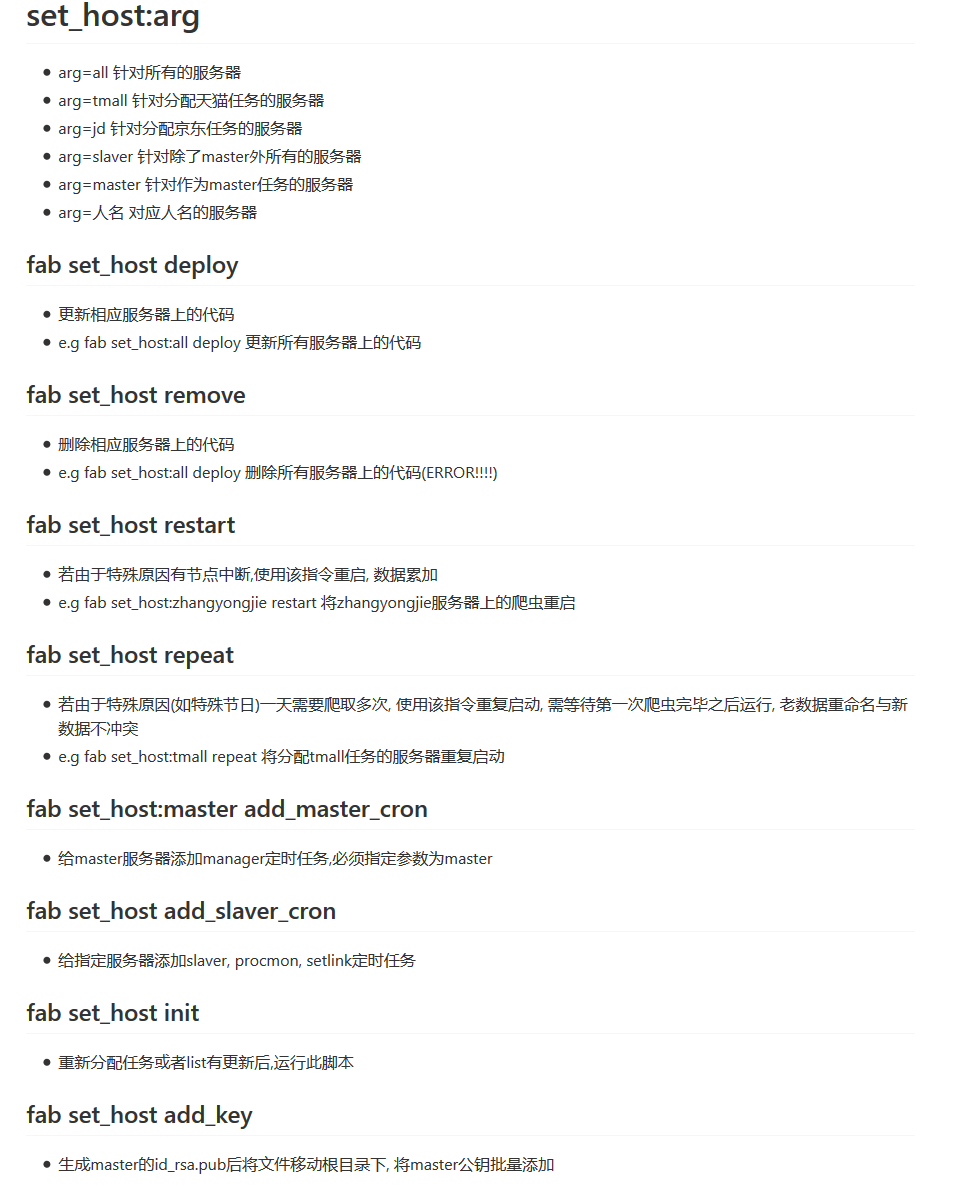
\includegraphics[width=6cm,height=7cm]{fsol_deploy1.png}
\end{center}
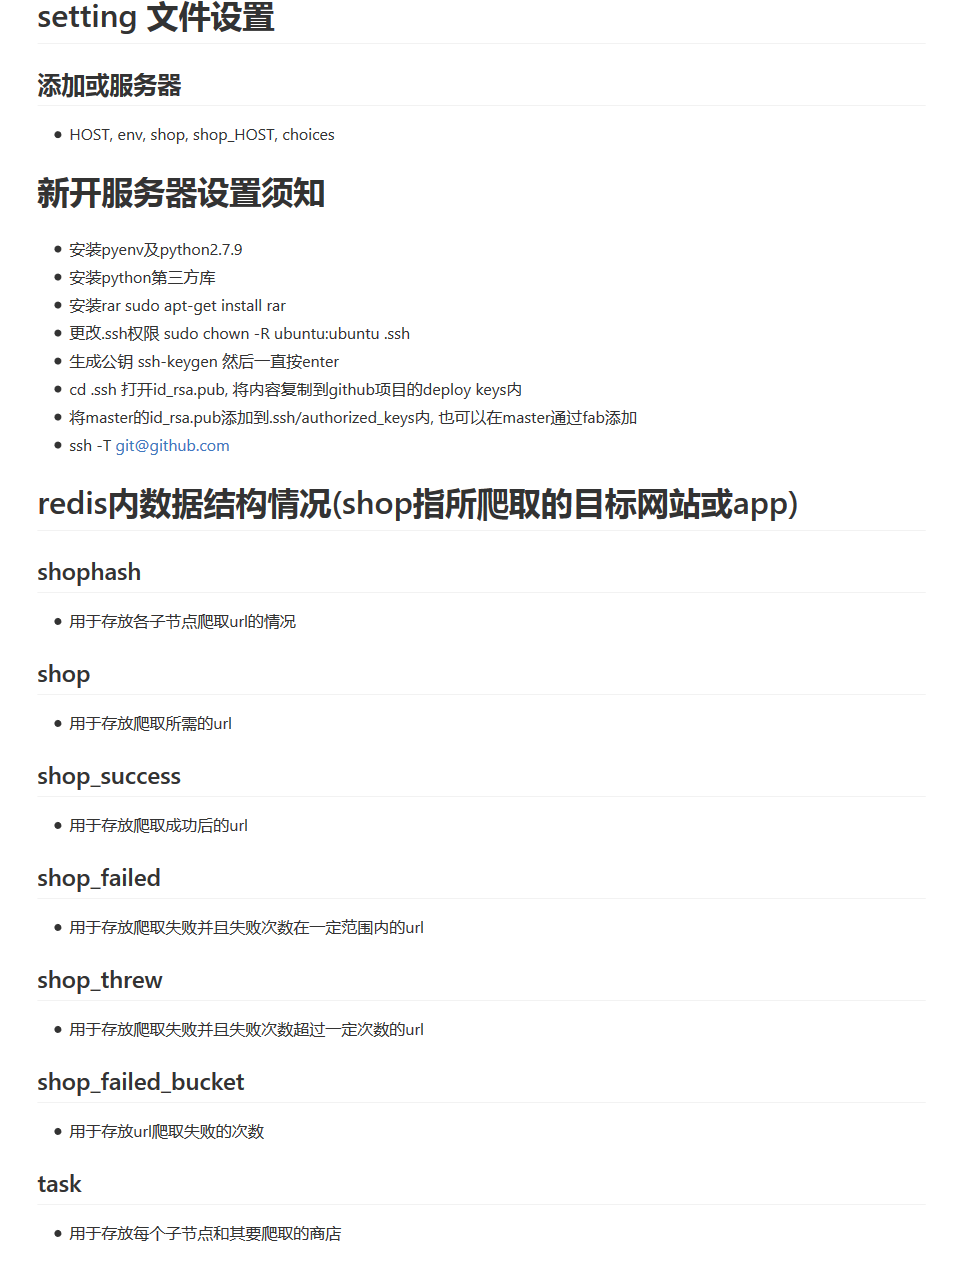
\includegraphics[width=6cm,height=7cm]{fsol_deploy2.png}
\end{multicols}
\end{frame}

\subsection{自动化管理}
\begin{frame}
\frametitle{自动化管理}
\begin{multicols}{2}
\begin{itemize}
\item  管理工具:slack——便捷的企业协作工作软件
\end{itemize}
\begin{center}
 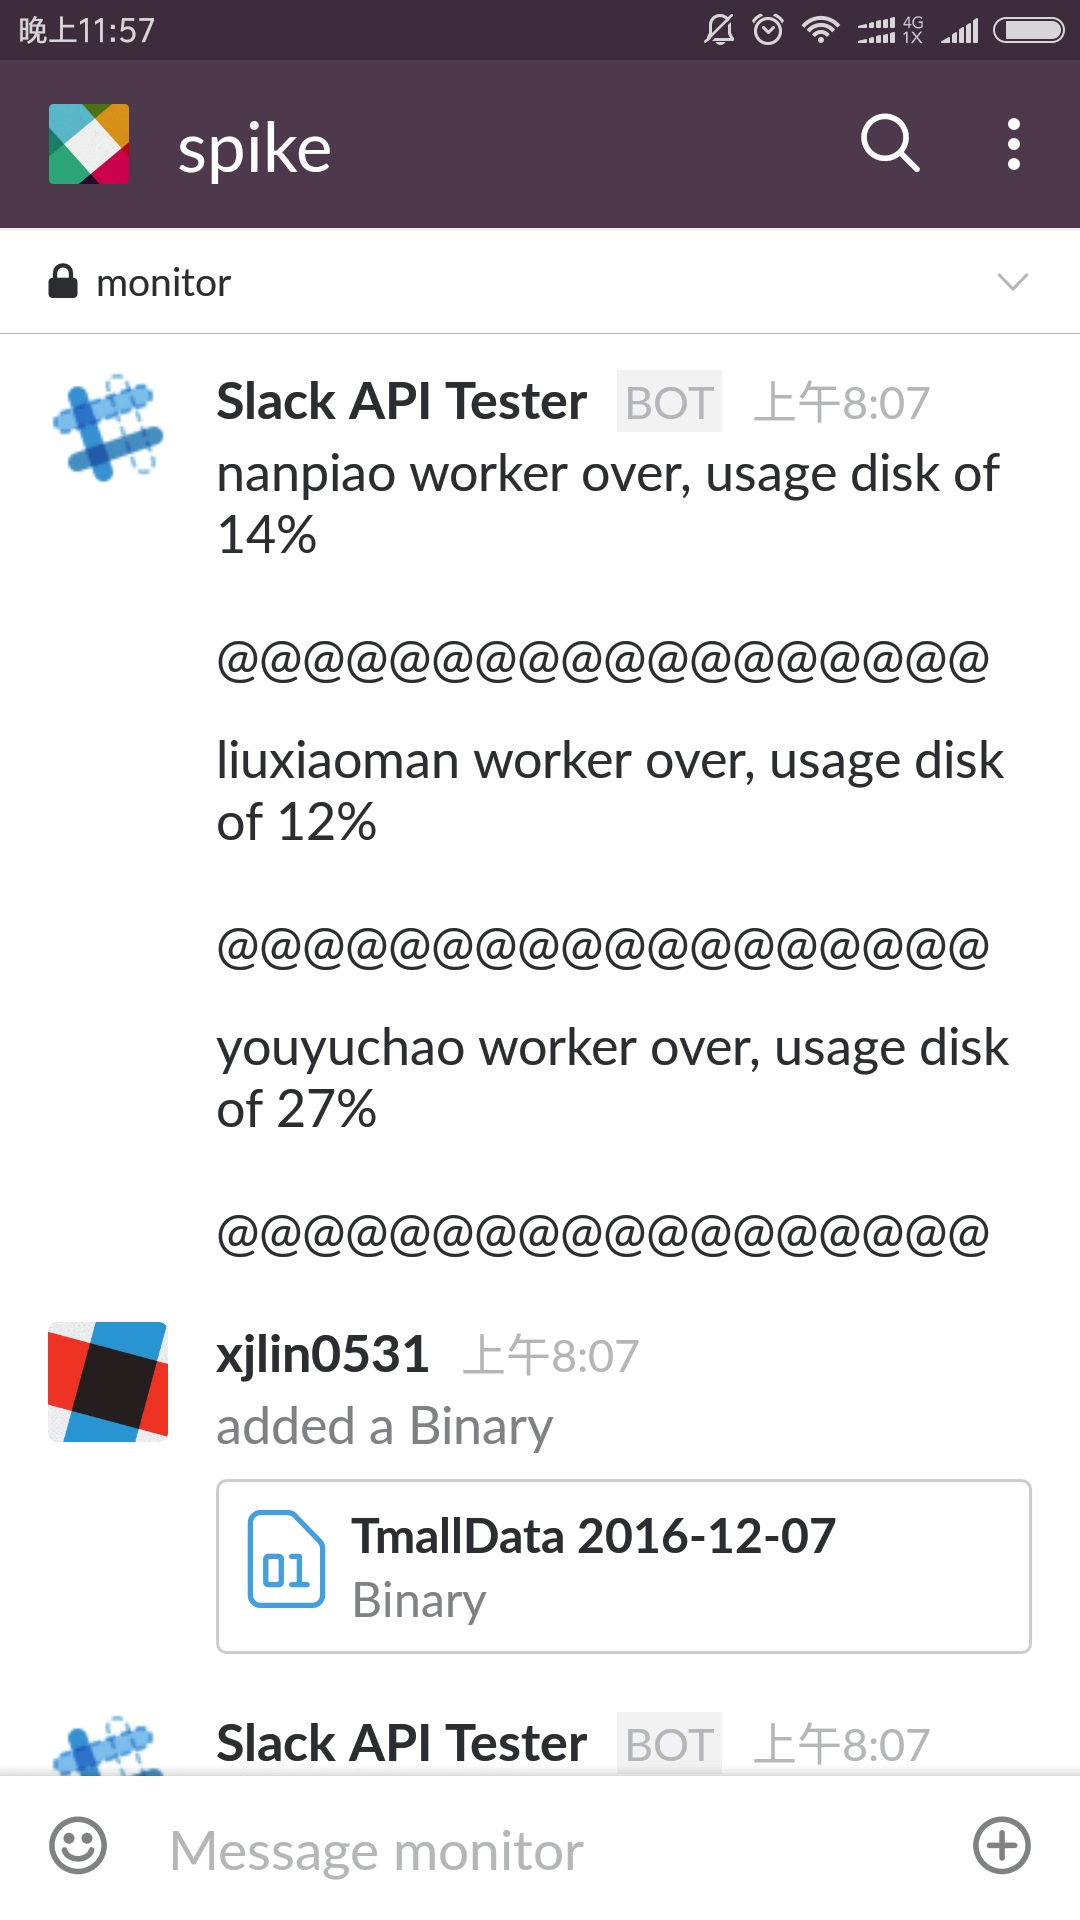
\includegraphics[width=4cm,height=7cm]{fsol_slack.png}
\end{center}
\end{multicols}
\end{frame}

\section{数据管理策略}
\subsection{日常管理}
\begin{frame}
\frametitle{日常管理}
\begin{itemize}
\item 管理任务:检查数据是否正常,将数据收理归类
\item Windows端管理:Winscp
\end{itemize}
\end{frame}

\subsection{后续管理}
\begin{frame}
\frametitle{后续管理}
\begin{itemize}
\item 任务:将原始数据整理归类,并输入数据库
\item 主要难点:原始数据量级过大时,硬件容易出现瓶颈
\end{itemize}
\end{frame}


\section{小结}
\begin{frame}
\frametitle{小结}
\begin{itemize}
  \item 主要优点:
  \begin{itemize}
  \item 操作难度极低,几乎不需要什么计算机基础
  \end{itemize}
  \item 待解决问题:
  \begin{itemize}
    \item 部署任务依然需要使用命令行
    \item 数据管理步骤仍然繁琐
  \end{itemize}
  \item 解决方案:
  \begin{itemize}
    \item 部署任务将会转移到slack上
    \item 直接把数据输入数据库,进一步减少操作复杂度
  \end{itemize}
\end{itemize}
\end{frame}

\begin{frame}
\begin{center}
  
\includegraphics[width=7cm,height=7cm]{CPP.jpg}
\end{center}
\end{frame}


\end{document}
